\documentclass[12pt,a4paper]{article}
\usepackage{graphicx}
\usepackage{amsmath}
\usepackage{bm}
\usepackage{interval}
\usepackage{amssymb}
\usepackage{float}
\usepackage{subfigure}
\usepackage[letterpaper,top=2cm,bottom=2cm,left=3cm,right=3cm,marginparwidth=1.75cm]{geometry}
\usepackage[colorlinks=true, allcolors=blue]{hyperref}

\title{DS Written Homework 2}
\author{Student ID: b10201054}

\begin{document}
\maketitle

\section{Binary Tree}


\begin{enumerate}
    \item[(a)] 
        \begin{figure}[H]
            \centering
            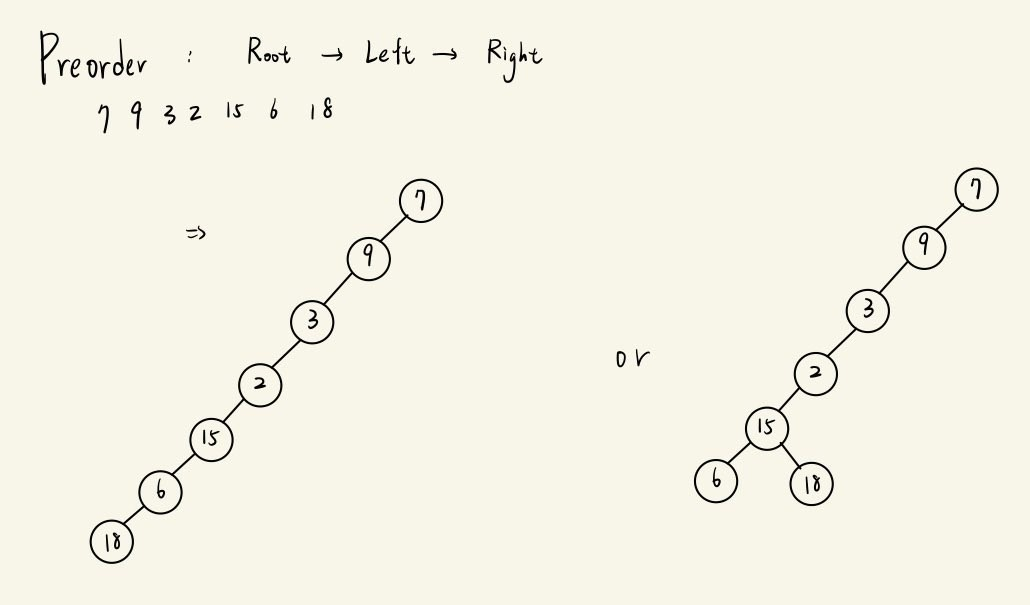
\includegraphics[width=0.7\linewidth]{Binarya.jpg}
            \caption{Binarytree}
        \end{figure}
        
    \item[(b)]
        \begin{figure}[H]
            \centering
            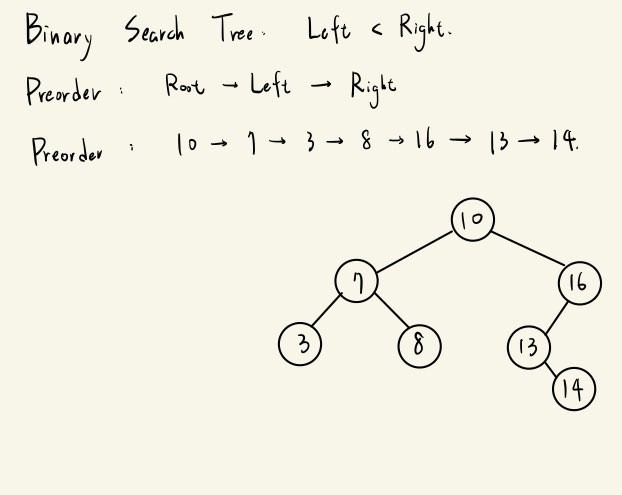
\includegraphics[width=0.7\linewidth]{Binaryb.jpg}
            \caption{Binarytree}
        \end{figure}
    
    \item[(c)]
        \begin{figure}[H]
            \centering
            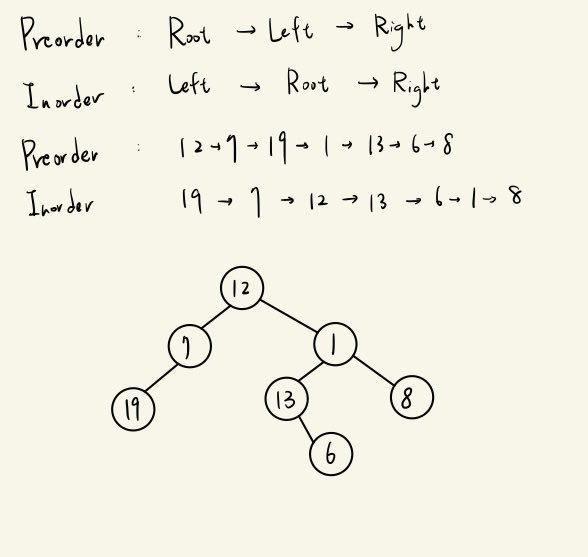
\includegraphics[width=0.7\linewidth]{Binaryc.jpg}
            \caption{Binarytree}
        \end{figure}
    
\end{enumerate}

\section{Recursion Problem}    

\begin{enumerate}
    \item[(a)]
        
    \item[(b)]
        
    
\end{enumerate}

\section{AVL Tree}    

\begin{enumerate}
    \item[(a)] 
        \begin{figure}[H]
            \centering
            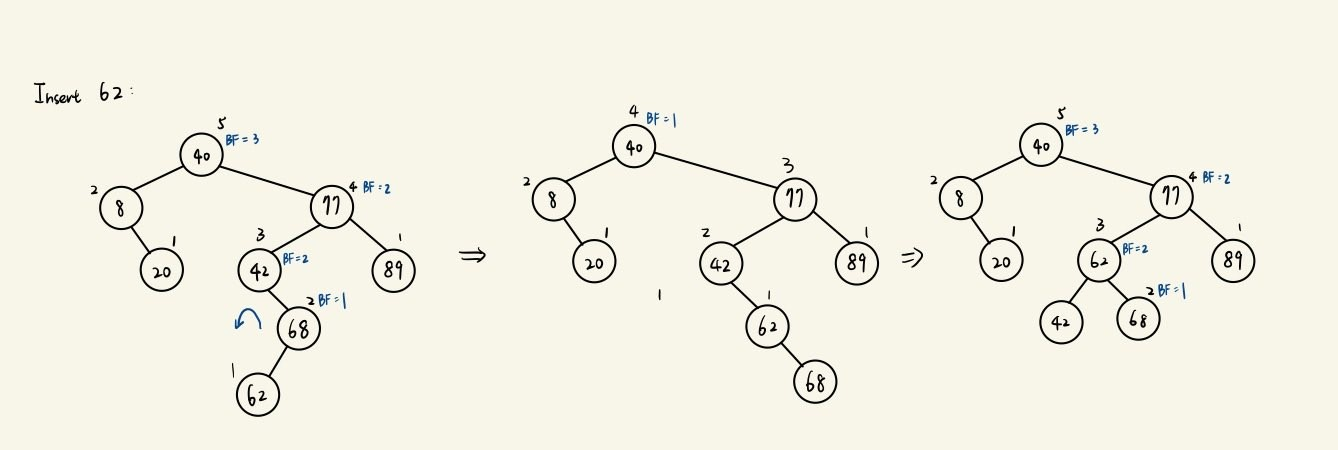
\includegraphics[width=0.8\linewidth]{AVLa.jpg}
            \caption{Binarytree}
        \end{figure}
    \item[(b)]
        \begin{figure}[H]
            \centering
            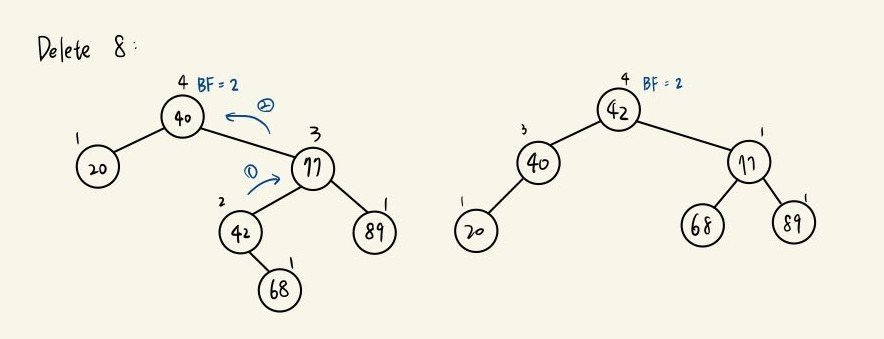
\includegraphics[width=0.8\linewidth]{AVLb.jpg}
            \caption{Binarytree}
        \end{figure}
    \item[(c)]
        The minimum height is $\left\lceil (\log_{2} (n+1))\right\rceil $.

        Since AVL Tree must follow the rule $\left\lvert left\_height - right\_height\right\rvert \leq 1$, the worst case of AVL Tree is Fibonacci Tree.
        Fibonacci tree gives us $T(0) = 0, T(1) = 1, T(h) = T(h-1) + T(h-2) +1$, where $h$ means the tree's height, and $T(h)$ means the number of nodes in the h-height Fibonacci Tree.
        In this recurrence relation, we can easily compute the general function $T(h) = \frac{(\phi^{h+2} - \varphi ^{h+2})}{\sqrt{5}} - 1$, where $\phi$ is golden ratio and $\varphi$ is its conjugate.
        
        In this case, we want to find h such that $T(h) = 493$. We can set $\varphi ^{h+2} = \epsilon$ since it's much more smaller than $\phi^{h+2}$. Then the equation will become
        \[
            T(h) = \frac{\phi^{h+2}}{\sqrt{5}} - \epsilon - 1 = 493
        \]
        After solving the equation, we have $h = \left\lfloor \log_{\phi} \sqrt{5}(494+\epsilon) - 2\right\rfloor $.
        After computing the $\left\lfloor \log_{\phi} \sqrt{5}(494+\epsilon) - 2\right\rfloor = 12$ and $\left\lceil (\log_{2} (494))\right\rceil = 9$, the possible heights is 9, 10, 11, 12.
\end{enumerate}

\section{Parentheses Balance Problem}

\begin{enumerate}
    \item[(a)] 
        
    \item[(b)]
        
    \item[(c)]
        
\end{enumerate}

\section{Complexity Analysis}

\begin{enumerate}
    \item[(a)] 
        Consider the recurrence relation
        \[
            \left\{
                \begin{matrix}
                    a_n &=& a_{n-2} + n\\
                    a_1 &=& k_1 (constant)\\
                    a_0 &=& k_0 (constant)
                \end{matrix}
            \right.
        \]
        If n is even, we have $a_n = a_0 + \sum_{k=1}^{\frac{n}{2}}k = a_0 + \frac{1}{2}\cdot\frac{n}{2}\cdot\frac{n+2}{2}$. Hence the complexity is $O(n^2)$.
    \item[(b)]
        Consider the recurrence relation
        \[
            \left\{
                \begin{matrix}
                    a_n &=& 2a_{n-1} + n\\
                    a_1 &=& k (constant)
                \end{matrix}
            \right.
        \]
        We have the general $a_n =2^{n-1}(a_1 + 3)$, which means the complexity is $O(2^n)$
    \item[(c)]
    Consider the recurrence relation
    \[
        \left\{
            \begin{matrix}
                (a_n+\frac{1}{4}) &=& 2(a_{n-1}+\frac{1}{4}) + 3(a_{n-2}+\frac{1}{4})\\
                a_1 &=& 1\\
                a_2 &=& 1
            \end{matrix}
        \right.
    \]
    After solving its characteristic equation $r^2 = 2r + 3$, we get two roots 3, -1.
    The general $a_n = C\cdot (3)^n + D\cdot (-1)^n$. Hence the complexity is $O(3^n)$
    \item[(d)]
        Consider the recurrence relation
        \[
            \left\{
                \begin{matrix}
                    a_n &=& 8a_{\frac{n}{4}} + \log n\\
                    a_1 &=& k (constant)
                \end{matrix}
            \right.
        \]
        The recurrence relation will give us $a_n = 8^{\log_{4} n} a_1 + O(\log n) = n^{\frac{3}{2}} + O(\log n)$.
        Since we know polynomial is growing faster than $\log$, $T(n)$ has time complexity $O(n^{\frac{3}{2}})$.
    \item[(e)] 
        $T(n) = T(\sqrt{n}) + 1$, assume that when m-th recurrence, $n^{\frac{1}{2^m}}\approx 1 + 10^{-6}$. In the m-th recurrence we have 
        \[
            T(n) = T(n^{\frac{1}{2^m}}) + m \approx m + 1
        \]
        Compute m:
        \[
                \log n = 2^{m}\log(1 + 10^{6}) \Rightarrow m = \log_{2}(\frac{\log n}{\log(1+10^{-6})})
        \]
        Hence, the complexity is $O(\log\log n)$
    \item[(f)]
        $T(n) = 3T(\sqrt{n}) + 1$, assume that when m-th recurrence, $n^{\frac{1}{2^m}}\approx 1 + 10^{-6}$. In the m-th recurrence we have 
        \[
            T(n) = 3^m\cdot T(n^{\frac{1}{2^m}}) + m \approx m + 3^m
        \]
        Compute m:
        \[
                \log n = 2^{m}\log(1 + 10^{6}) \Rightarrow m = \log_{2}(\frac{\log n}{\log(1+10^{-6})})
        \]
        Then $3^m$:
        \[
                3^{\log_{2}(\frac{\log n}{\log(1+10^{-6})})} = \log_{2}3\frac{\log n}{\log(1+10^{-6})} 
        \]
        Hence, the complexity is $O(\log n)$
\end{enumerate}

\section{Problem 6}


\end{document}
